\documentclass[1p]{elsarticle_modified}
%\bibliographystyle{elsarticle-num}

%\usepackage[colorlinks]{hyperref}
%\usepackage{abbrmath_seonhwa} %\Abb, \Ascr, \Acal ,\Abf, \Afrak
\usepackage{amsfonts}
\usepackage{amssymb}
\usepackage{amsmath}
\usepackage{amsthm}
\usepackage{scalefnt}
\usepackage{amsbsy}
\usepackage{kotex}
\usepackage{caption}
\usepackage{subfig}
\usepackage{color}
\usepackage{graphicx}
\usepackage{xcolor} %% white, black, red, green, blue, cyan, magenta, yellow
\usepackage{float}
\usepackage{setspace}
\usepackage{hyperref}

\usepackage{tikz}
\usetikzlibrary{arrows}

\usepackage{multirow}
\usepackage{array} % fixed length table
\usepackage{hhline}

%%%%%%%%%%%%%%%%%%%%%
\makeatletter
\renewcommand*\env@matrix[1][\arraystretch]{%
	\edef\arraystretch{#1}%
	\hskip -\arraycolsep
	\let\@ifnextchar\new@ifnextchar
	\array{*\c@MaxMatrixCols c}}
\makeatother %https://tex.stackexchange.com/questions/14071/how-can-i-increase-the-line-spacing-in-a-matrix
%%%%%%%%%%%%%%%

\usepackage[normalem]{ulem}

\newcommand{\msout}[1]{\ifmmode\text{\sout{\ensuremath{#1}}}\else\sout{#1}\fi}
%SOURCE: \msout is \stkout macro in https://tex.stackexchange.com/questions/20609/strikeout-in-math-mode

\newcommand{\cancel}[1]{
	\ifmmode
	{\color{red}\msout{#1}}
	\else
	{\color{red}\sout{#1}}
	\fi
}

\newcommand{\add}[1]{
	{\color{blue}\uwave{#1}}
}

\newcommand{\replace}[2]{
	\ifmmode
	{\color{red}\msout{#1}}{\color{blue}\uwave{#2}}
	\else
	{\color{red}\sout{#1}}{\color{blue}\uwave{#2}}
	\fi
}

\newcommand{\Sol}{\mathcal{S}} %segment
\newcommand{\D}{D} %diagram
\newcommand{\A}{\mathcal{A}} %arc


%%%%%%%%%%%%%%%%%%%%%%%%%%%%%5 test

\def\sl{\operatorname{\textup{SL}}(2,\Cbb)}
\def\psl{\operatorname{\textup{PSL}}(2,\Cbb)}
\def\quan{\mkern 1mu \triangleright \mkern 1mu}

\theoremstyle{definition}
\newtheorem{thm}{Theorem}[section]
\newtheorem{prop}[thm]{Proposition}
\newtheorem{lem}[thm]{Lemma}
\newtheorem{ques}[thm]{Question}
\newtheorem{cor}[thm]{Corollary}
\newtheorem{defn}[thm]{Definition}
\newtheorem{exam}[thm]{Example}
\newtheorem{rmk}[thm]{Remark}
\newtheorem{alg}[thm]{Algorithm}

\newcommand{\I}{\sqrt{-1}}
\begin{document}

%\begin{frontmatter}
%
%\title{Boundary parabolic representations of knots up to 8 crossings}
%
%%% Group authors per affiliation:
%\author{Yunhi Cho} 
%\address{Department of Mathematics, University of Seoul, Seoul, Korea}
%\ead{yhcho@uos.ac.kr}
%
%
%\author{Seonhwa Kim} %\fnref{s_kim}}
%\address{Center for Geometry and Physics, Institute for Basic Science, Pohang, 37673, Korea}
%\ead{ryeona17@ibs.re.kr}
%
%\author{Hyuk Kim}
%\address{Department of Mathematical Sciences, Seoul National University, Seoul 08826, Korea}
%\ead{hyukkim@snu.ac.kr}
%
%\author{Seokbeom Yoon}
%\address{Department of Mathematical Sciences, Seoul National University, Seoul, 08826,  Korea}
%\ead{sbyoon15@snu.ac.kr}
%
%\begin{abstract}
%We find all boundary parabolic representation of knots up to 8 crossings.
%
%\end{abstract}
%\begin{keyword}
%    \MSC[2010] 57M25 
%\end{keyword}
%
%\end{frontmatter}

%\linenumbers
%\tableofcontents
%
\newcommand\colored[1]{\textcolor{white}{\rule[-0.35ex]{0.8em}{1.4ex}}\kern-0.8em\color{red} #1}%
%\newcommand\colored[1]{\textcolor{white}{ #1}\kern-2.17ex	\textcolor{white}{ #1}\kern-1.81ex	\textcolor{white}{ #1}\kern-2.15ex\color{red}#1	}

{\Large $\underline{11a_{231}~(K11a_{231})}$}

\setlength{\tabcolsep}{10pt}
\renewcommand{\arraystretch}{1.6}
\vspace{1cm}\begin{tabular}{m{100pt}>{\centering\arraybackslash}m{274pt}}
\multirow{5}{120pt}{
	\centering
	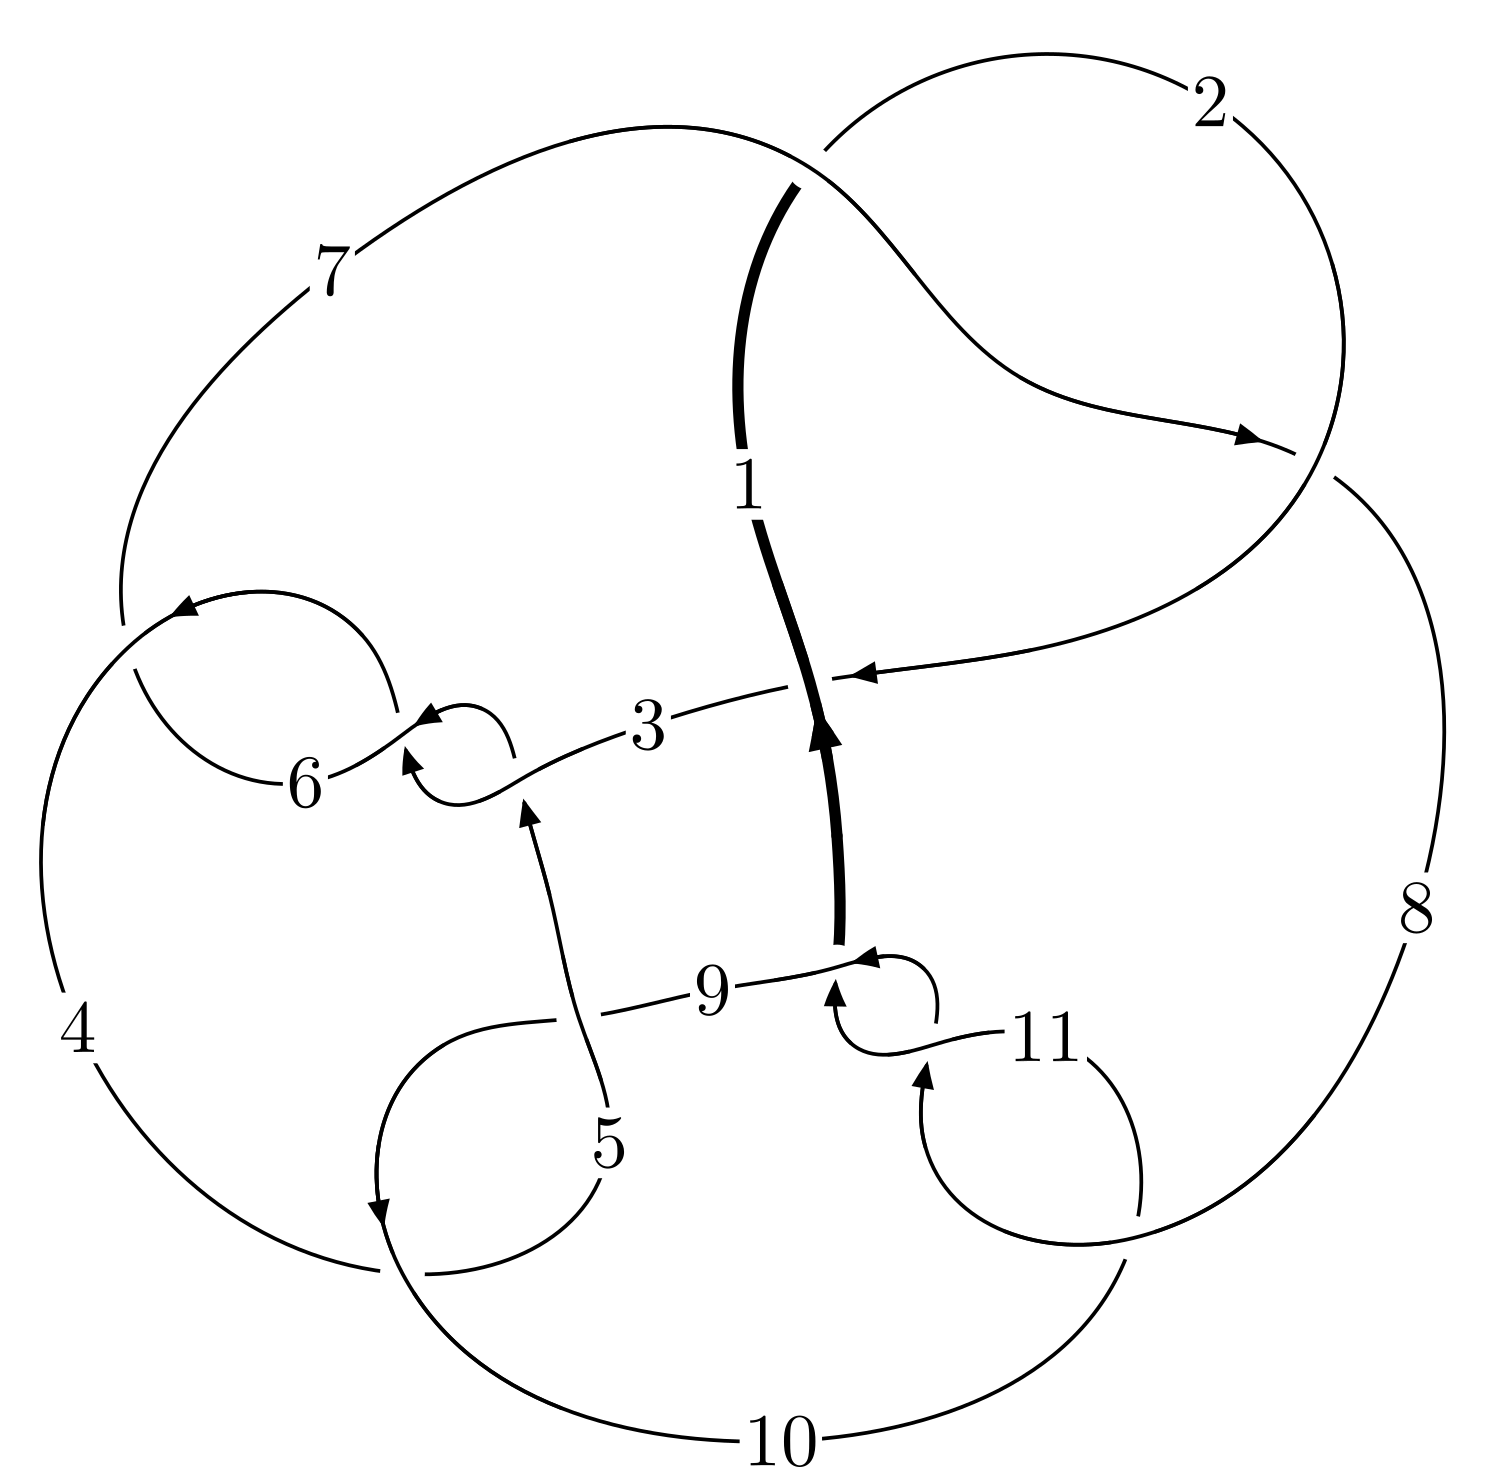
\includegraphics[width=112pt]{../../../GIT/diagram.site/Diagrams/png/480_11a_231.png}\\
\ \ \ A knot diagram\footnotemark}&
\allowdisplaybreaks
\textbf{Linearized knot diagam} \\
\cline{2-2}
 &
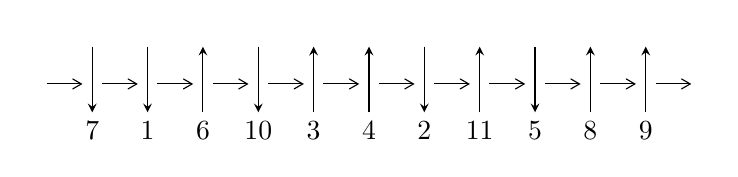
\begin{tikzpicture}[x=20pt, y=17pt]
	% nodes
	\node (C0) at (0, 0) {};
	\node (C1) at (1, 0) {};
	\node (C1U) at (1, +1) {};
	\node (C1D) at (1, -1) {7};

	\node (C2) at (2, 0) {};
	\node (C2U) at (2, +1) {};
	\node (C2D) at (2, -1) {1};

	\node (C3) at (3, 0) {};
	\node (C3U) at (3, +1) {};
	\node (C3D) at (3, -1) {6};

	\node (C4) at (4, 0) {};
	\node (C4U) at (4, +1) {};
	\node (C4D) at (4, -1) {10};

	\node (C5) at (5, 0) {};
	\node (C5U) at (5, +1) {};
	\node (C5D) at (5, -1) {3};

	\node (C6) at (6, 0) {};
	\node (C6U) at (6, +1) {};
	\node (C6D) at (6, -1) {4};

	\node (C7) at (7, 0) {};
	\node (C7U) at (7, +1) {};
	\node (C7D) at (7, -1) {2};

	\node (C8) at (8, 0) {};
	\node (C8U) at (8, +1) {};
	\node (C8D) at (8, -1) {11};

	\node (C9) at (9, 0) {};
	\node (C9U) at (9, +1) {};
	\node (C9D) at (9, -1) {5};

	\node (C10) at (10, 0) {};
	\node (C10U) at (10, +1) {};
	\node (C10D) at (10, -1) {8};

	\node (C11) at (11, 0) {};
	\node (C11U) at (11, +1) {};
	\node (C11D) at (11, -1) {9};
	\node (C12) at (12, 0) {};

	% arrows
	\draw[->,>={angle 60}]
	(C0) edge (C1) (C1) edge (C2) (C2) edge (C3) (C3) edge (C4) (C4) edge (C5) (C5) edge (C6) (C6) edge (C7) (C7) edge (C8) (C8) edge (C9) (C9) edge (C10) (C10) edge (C11) (C11) edge (C12) ;	\draw[->,>=stealth]
	(C1U) edge (C1D) (C2U) edge (C2D) (C3D) edge (C3U) (C4U) edge (C4D) (C5D) edge (C5U) (C6D) edge (C6U) (C7U) edge (C7D) (C8D) edge (C8U) (C9U) edge (C9D) (C10D) edge (C10U) (C11D) edge (C11U) ;
	\end{tikzpicture} \\
\hhline{~~} \\& 
\textbf{Solving Sequence} \\ \cline{2-2} 
 &
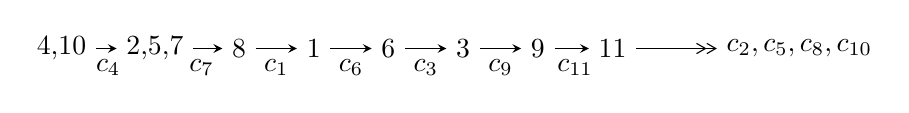
\begin{tikzpicture}[x=27pt, y=7pt]
	% node
	\node (A0) at (-1/8, 0) {4,10};
	\node (A1) at (9/8, 0) {2,5,7};
	\node (A2) at (9/4, 0) {8};
	\node (A3) at (13/4, 0) {1};
	\node (A4) at (17/4, 0) {6};
	\node (A5) at (21/4, 0) {3};
	\node (A6) at (25/4, 0) {9};
	\node (A7) at (29/4, 0) {11};
	\node (C1) at (1/2, -1) {$c_{4}$};
	\node (C2) at (7/4, -1) {$c_{7}$};
	\node (C3) at (11/4, -1) {$c_{1}$};
	\node (C4) at (15/4, -1) {$c_{6}$};
	\node (C5) at (19/4, -1) {$c_{3}$};
	\node (C6) at (23/4, -1) {$c_{9}$};
	\node (C7) at (27/4, -1) {$c_{11}$};
	\node (A8) at (39/4, 0) {$c_{2},c_{5},c_{8},c_{10}$};

	% edge
	\draw[->,>=stealth]	
	(A0) edge (A1) (A1) edge (A2) (A2) edge (A3) (A3) edge (A4) (A4) edge (A5) (A5) edge (A6) (A6) edge (A7) ;
	\draw[->>,>={angle 60}]	
	(A7) edge (A8);
\end{tikzpicture} \\ 

\end{tabular} \\

\footnotetext{
The image of knot diagram is generated by the software ``\textbf{Draw programme}" developed by Andrew Bartholomew(\url{http://www.layer8.co.uk/maths/draw/index.htm\#Running-draw}), where we modified some parts for our purpose(\url{https://github.com/CATsTAILs/LinksPainter}).
}\phantom \\ \newline 
\centering \textbf{Ideals for irreducible components\footnotemark of $X_{\text{par}}$} 
 
\begin{align*}
I^u_{1}&=\langle 
49503754 u^{16}-103286795 u^{15}+\cdots+3447876362 d-235456666,\\
\phantom{I^u_{1}}&\phantom{= \langle  }58457271 u^{16}-270451180 u^{15}+\cdots+13791505448 c-14346071104,\\
\phantom{I^u_{1}}&\phantom{= \langle  }31318034 u^{16}-423514703 u^{15}+\cdots+6895752724 b-2520805844,\\
\phantom{I^u_{1}}&\phantom{= \langle  }630201461 u^{16}-1197766854 u^{15}+\cdots+13791505448 a-18642484192,\;u^{17}-2 u^{16}+\cdots-4 u^2+8\rangle \\
I^u_{2}&=\langle 
4 u^6 a+14 u^5 a-3 u^6+26 u^4 a-3 u^5+26 u^3 a-2 u^4+8 u^2 a+3 u^3-12 a u+9 u^2+10 d-14 a+9 u+8,\\
\phantom{I^u_{2}}&\phantom{= \langle  }3 u^6 a+3 u^5 a- u^6+2 u^4 a+4 u^5-3 u^3 a+11 u^4-9 u^2 a+21 u^3-9 a u+18 u^2+10 c-8 a+8 u+1,\\
\phantom{I^u_{2}}&\phantom{= \langle  }- u^5-2 u^4-3 u^3+a u-2 u^2+b- u,\\
\phantom{I^u_{2}}&\phantom{= \langle  }-4 u^6-2 u^4 a-9 u^5-4 u^3 a-15 u^4-6 u^2 a-10 u^3+2 a^2-4 a u-3 u^2-2 a+7 u+7,\\
\phantom{I^u_{2}}&\phantom{= \langle  }u^7+3 u^6+6 u^5+7 u^4+5 u^3+u^2-2 u-2\rangle \\
I^u_{3}&=\langle 
u^3+d+u,\;c+u,\;u^4-2 u^2 a- u^3+a u+u^2+b-2 a-1,\\
\phantom{I^u_{3}}&\phantom{= \langle  }- u^4 a+2 u^3 a-3 u^2 a+u^3+a^2+2 a u- u^2- a+2 u-1,\;u^5- u^4+2 u^3- u^2+u-1\rangle \\
I^u_{4}&=\langle 
-6 u^4 a+u^3 a+2 u^4-15 u^2 a-8 u^3+5 a u+5 u^2+23 d+2 a-17 u+7,\\
\phantom{I^u_{4}}&\phantom{= \langle  }-2 u^4 a-15 u^3 a-7 u^4-5 u^2 a+5 u^3-6 a u-6 u^2+23 c-7 a-21 u+10,\\
\phantom{I^u_{4}}&\phantom{= \langle  }-4 u^4 a+16 u^3 a+9 u^4-10 u^2 a-13 u^3+11 a u+11 u^2+23 b-14 a+4 u-3,\\
\phantom{I^u_{4}}&\phantom{= \langle  }- u^4 a+2 u^4- u^2 a+u^3+a^2-2 a u+u^2- a+4 u+1,\;u^5- u^4+2 u^3- u^2+u-1\rangle \\
I^u_{5}&=\langle 
u^3+d+u,\;c+u,\;- u^4+u^3- u^2+b-1,\;- u^4- u^2+a-1,\;u^5- u^4+2 u^3- u^2+u-1\rangle \\
\\
I^v_{1}&=\langle 
a,\;d+1,\;c+a,\;b-1,\;v+1\rangle \\
I^v_{2}&=\langle 
a,\;d,\;c-1,\;b+1,\;v-1\rangle \\
I^v_{3}&=\langle 
a,\;d+1,\;c+a-1,\;b-1,\;v-1\rangle \\
I^v_{4}&=\langle 
c,\;d+1,\;c b+a-1,\;c v+a v- c- v,\;b v- v+1\rangle \\
\end{align*}
\raggedright * 8 irreducible components of $\dim_{\mathbb{C}}=0$, with total 59 representations.\\
\raggedright * 1 irreducible components of $\dim_{\mathbb{C}}=1$ \\
\footnotetext{All coefficients of polynomials are rational numbers. But the coefficients are sometimes approximated in decimal forms when there is not enough margin.}
\newpage
\renewcommand{\arraystretch}{1}
\centering \section*{I. $I^u_{1}= \langle 4.95\times10^{7} u^{16}-1.03\times10^{8} u^{15}+\cdots+3.45\times10^{9} d-2.35\times10^{8},\;5.85\times10^{7} u^{16}-2.70\times10^{8} u^{15}+\cdots+1.38\times10^{10} c-1.43\times10^{10},\;3.13\times10^{7} u^{16}-4.24\times10^{8} u^{15}+\cdots+6.90\times10^{9} b-2.52\times10^{9},\;6.30\times10^{8} u^{16}-1.20\times10^{9} u^{15}+\cdots+1.38\times10^{10} a-1.86\times10^{10},\;u^{17}-2 u^{16}+\cdots-4 u^2+8 \rangle$}
\flushleft \textbf{(i) Arc colorings}\\
\begin{tabular}{m{7pt} m{180pt} m{7pt} m{180pt} }
\flushright $a_{4}=$&$\begin{pmatrix}1\\0\end{pmatrix}$ \\
\flushright $a_{10}=$&$\begin{pmatrix}0\\u\end{pmatrix}$ \\
\flushright $a_{2}=$&$\begin{pmatrix}-0.0456949 u^{16}+0.0868482 u^{15}+\cdots+0.0108537 u+1.35174\\-0.00454164 u^{16}+0.0614167 u^{15}+\cdots+1.35174 u+0.365559\end{pmatrix}$ \\
\flushright $a_{5}=$&$\begin{pmatrix}1\\u^2\end{pmatrix}$ \\
\flushright $a_{7}=$&$\begin{pmatrix}-0.00423864 u^{16}+0.0196100 u^{15}+\cdots-0.366884 u+1.04021\\-0.0143578 u^{16}+0.0299566 u^{15}+\cdots-0.201558 u+0.0682903\end{pmatrix}$ \\
\flushright $a_{8}=$&$\begin{pmatrix}0.00853629 u^{16}-0.00271483 u^{15}+\cdots-0.843158 u+0.201558\\-0.0111327 u^{16}+0.00527464 u^{15}+\cdots-1.04021 u-0.0339091\end{pmatrix}$ \\
\flushright $a_{1}=$&$\begin{pmatrix}0.0196690 u^{16}-0.00798947 u^{15}+\cdots+0.197053 u+0.235467\\0.00442501 u^{16}+0.0219877 u^{15}+\cdots+0.882859 u-0.216879\end{pmatrix}$ \\
\flushright $a_{6}=$&$\begin{pmatrix}0.0101191 u^{16}-0.0103467 u^{15}+\cdots-0.165326 u+0.971920\\-0.0143578 u^{16}+0.0299566 u^{15}+\cdots-0.201558 u+0.0682903\end{pmatrix}$ \\
\flushright $a_{3}=$&$\begin{pmatrix}0.0101191 u^{16}-0.0103467 u^{15}+\cdots-0.165326 u+0.971920\\0.0191724 u^{16}-0.0450506 u^{15}+\cdots+0.120605 u-0.147423\end{pmatrix}$ \\
\flushright $a_{9}=$&$\begin{pmatrix}u\\u^3+u\end{pmatrix}$ \\
\flushright $a_{11}=$&$\begin{pmatrix}0.0184279 u^{16}-0.0176833 u^{15}+\cdots+0.128762 u+0.120605\\0.00318587 u^{16}-0.0118199 u^{15}+\cdots+0.824498 u-0.234332\end{pmatrix}$\\ \flushright $a_{11}=$&$\begin{pmatrix}0.0184279 u^{16}-0.0176833 u^{15}+\cdots+0.128762 u+0.120605\\0.00318587 u^{16}-0.0118199 u^{15}+\cdots+0.824498 u-0.234332\end{pmatrix}$\\&\end{tabular}
\flushleft \textbf{(ii) Obstruction class $= -1$}\\~\\
\flushleft \textbf{(iii) Cusp Shapes $= \frac{975451789}{3447876362} u^{16}-\frac{210120269}{3447876362} u^{15}+\cdots+\frac{8037027246}{1723938181} u-\frac{2146878348}{1723938181}$}\\~\\
\newpage\renewcommand{\arraystretch}{1}
\flushleft \textbf{(iv) u-Polynomials at the component}\newline \\
\begin{tabular}{m{50pt}|m{274pt}}
Crossings & \hspace{64pt}u-Polynomials at each crossing \\
\hline $$\begin{aligned}c_{1},c_{7}\end{aligned}$$&$\begin{aligned}
&u^{17}-2 u^{16}+\cdots-8 u+4
\end{aligned}$\\
\hline $$\begin{aligned}c_{2}\end{aligned}$$&$\begin{aligned}
&u^{17}+6 u^{16}+\cdots+88 u+16
\end{aligned}$\\
\hline $$\begin{aligned}c_{3},c_{5},c_{6}\\c_{8},c_{10},c_{11}\end{aligned}$$&$\begin{aligned}
&u^{17}+2 u^{16}+\cdots+3 u+1
\end{aligned}$\\
\hline $$\begin{aligned}c_{4},c_{9}\end{aligned}$$&$\begin{aligned}
&u^{17}-2 u^{16}+\cdots-4 u^2+8
\end{aligned}$\\
\hline
\end{tabular}\\~\\
\newpage\renewcommand{\arraystretch}{1}
\flushleft \textbf{(v) Riley Polynomials at the component}\newline \\
\begin{tabular}{m{50pt}|m{274pt}}
Crossings & \hspace{64pt}Riley Polynomials at each crossing \\
\hline $$\begin{aligned}c_{1},c_{7}\end{aligned}$$&$\begin{aligned}
&y^{17}-6 y^{16}+\cdots+88 y-16
\end{aligned}$\\
\hline $$\begin{aligned}c_{2}\end{aligned}$$&$\begin{aligned}
&y^{17}+10 y^{16}+\cdots+288 y-256
\end{aligned}$\\
\hline $$\begin{aligned}c_{3},c_{5},c_{6}\\c_{8},c_{10},c_{11}\end{aligned}$$&$\begin{aligned}
&y^{17}-20 y^{16}+\cdots+27 y-1
\end{aligned}$\\
\hline $$\begin{aligned}c_{4},c_{9}\end{aligned}$$&$\begin{aligned}
&y^{17}+6 y^{16}+\cdots+64 y-64
\end{aligned}$\\
\hline
\end{tabular}\\~\\
\newpage\flushleft \textbf{(vi) Complex Volumes and Cusp Shapes}
$$\begin{array}{c|c|c}  
\text{Solutions to }I^u_{1}& \I (\text{vol} + \sqrt{-1}CS) & \text{Cusp shape}\\
 \hline 
\begin{aligned}
u &= \phantom{-}0.679716 + 0.561358 I \\
a &= \phantom{-}0.75464 + 1.62593 I \\
b &= -0.39979 + 1.52879 I \\
c &= \phantom{-}0.849883 + 1.063640 I \\
d &= \phantom{-}0.073472 + 0.578699 I\end{aligned}
 & -3.14388 + 1.09865 I & -5.52136 - 1.09882 I \\ \hline\begin{aligned}
u &= \phantom{-}0.679716 - 0.561358 I \\
a &= \phantom{-}0.75464 - 1.62593 I \\
b &= -0.39979 - 1.52879 I \\
c &= \phantom{-}0.849883 - 1.063640 I \\
d &= \phantom{-}0.073472 - 0.578699 I\end{aligned}
 & -3.14388 - 1.09865 I & -5.52136 + 1.09882 I \\ \hline\begin{aligned}
u &= \phantom{-}0.555749 + 1.023030 I \\
a &= -1.22318 - 0.96405 I \\
b &= \phantom{-}0.30647 - 1.78712 I \\
c &= \phantom{-}0.306715 + 1.153640 I \\
d &= -0.260592 + 0.795594 I\end{aligned}
 & -1.71782 - 5.90288 I & -0.75718 + 7.23695 I \\ \hline\begin{aligned}
u &= \phantom{-}0.555749 - 1.023030 I \\
a &= -1.22318 + 0.96405 I \\
b &= \phantom{-}0.30647 + 1.78712 I \\
c &= \phantom{-}0.306715 - 1.153640 I \\
d &= -0.260592 - 0.795594 I\end{aligned}
 & -1.71782 + 5.90288 I & -0.75718 - 7.23695 I \\ \hline\begin{aligned}
u &= -1.247530 + 0.318357 I \\
a &= -0.254428 + 0.248211 I \\
b &= \phantom{-}0.238386 - 0.390648 I \\
c &= -1.033850 + 0.177824 I \\
d &= -1.44180 + 0.15237 I\end{aligned}
 & \phantom{-}8.60033 - 1.91429 I & \phantom{-}8.38805 + 0.33236 I \\ \hline\begin{aligned}
u &= -1.247530 - 0.318357 I \\
a &= -0.254428 - 0.248211 I \\
b &= \phantom{-}0.238386 + 0.390648 I \\
c &= -1.033850 - 0.177824 I \\
d &= -1.44180 - 0.15237 I\end{aligned}
 & \phantom{-}8.60033 + 1.91429 I & \phantom{-}8.38805 - 0.33236 I\\
 \hline 
 \end{array}$$\newpage$$\begin{array}{c|c|c}  
\text{Solutions to }I^u_{1}& \I (\text{vol} + \sqrt{-1}CS) & \text{Cusp shape}\\
 \hline 
\begin{aligned}
u &= -0.022849 + 0.695780 I \\
a &= \phantom{-}0.596447 - 0.521515 I \\
b &= \phantom{-}0.349231 + 0.426912 I \\
c &= \phantom{-}0.070481 - 0.342332 I \\
d &= -0.556553 - 0.244029 I\end{aligned}
 & \phantom{-}0.88275 + 1.29794 I & \phantom{-}5.86581 - 6.22804 I \\ \hline\begin{aligned}
u &= -0.022849 - 0.695780 I \\
a &= \phantom{-}0.596447 + 0.521515 I \\
b &= \phantom{-}0.349231 - 0.426912 I \\
c &= \phantom{-}0.070481 + 0.342332 I \\
d &= -0.556553 + 0.244029 I\end{aligned}
 & \phantom{-}0.88275 - 1.29794 I & \phantom{-}5.86581 + 6.22804 I \\ \hline\begin{aligned}
u &= \phantom{-}1.235140 + 0.560024 I \\
a &= -1.37636 - 0.88777 I \\
b &= -1.20283 - 1.86731 I \\
c &= -1.030900 - 0.315398 I \\
d &= -1.43635 - 0.27040 I\end{aligned}
 & \phantom{-}6.85439 + 7.49245 I & \phantom{-}6.04980 - 5.00652 I \\ \hline\begin{aligned}
u &= \phantom{-}1.235140 - 0.560024 I \\
a &= -1.37636 + 0.88777 I \\
b &= -1.20283 + 1.86731 I \\
c &= -1.030900 + 0.315398 I \\
d &= -1.43635 + 0.27040 I\end{aligned}
 & \phantom{-}6.85439 - 7.49245 I & \phantom{-}6.04980 + 5.00652 I \\ \hline\begin{aligned}
u &= -0.66454 + 1.33308 I \\
a &= -0.189517 - 0.255094 I \\
b &= \phantom{-}0.466001 - 0.083122 I \\
c &= \phantom{-}0.052946 + 1.267480 I \\
d &= \phantom{-}1.48587 + 0.32095 I\end{aligned}
 & \phantom{-}11.9481 + 8.6770 I & \phantom{-}9.06927 - 4.38269 I \\ \hline\begin{aligned}
u &= -0.66454 - 1.33308 I \\
a &= -0.189517 + 0.255094 I \\
b &= \phantom{-}0.466001 + 0.083122 I \\
c &= \phantom{-}0.052946 - 1.267480 I \\
d &= \phantom{-}1.48587 - 0.32095 I\end{aligned}
 & \phantom{-}11.9481 - 8.6770 I & \phantom{-}9.06927 + 4.38269 I\\
 \hline 
 \end{array}$$\newpage$$\begin{array}{c|c|c}  
\text{Solutions to }I^u_{1}& \I (\text{vol} + \sqrt{-1}CS) & \text{Cusp shape}\\
 \hline 
\begin{aligned}
u &= \phantom{-}0.79652 + 1.26851 I \\
a &= \phantom{-}0.52130 + 1.70360 I \\
b &= -1.74580 + 2.01822 I \\
c &= \phantom{-}0.18365 - 1.46954 I \\
d &= \phantom{-}1.45618 - 0.38779 I\end{aligned}
 & \phantom{-}9.1924 - 14.7354 I & \phantom{-}6.16899 + 8.15927 I \\ \hline\begin{aligned}
u &= \phantom{-}0.79652 - 1.26851 I \\
a &= \phantom{-}0.52130 - 1.70360 I \\
b &= -1.74580 - 2.01822 I \\
c &= \phantom{-}0.18365 + 1.46954 I \\
d &= \phantom{-}1.45618 + 0.38779 I\end{aligned}
 & \phantom{-}9.1924 + 14.7354 I & \phantom{-}6.16899 - 8.15927 I \\ \hline\begin{aligned}
u &= -0.11728 + 1.54547 I \\
a &= -0.380984 + 0.529958 I \\
b &= -0.774348 - 0.650953 I \\
c &= -0.113527 + 0.217154 I \\
d &= \phantom{-}1.58385 + 0.05558 I\end{aligned}
 & \phantom{-}15.7365 + 3.2760 I & \phantom{-}10.07807 - 2.58290 I \\ \hline\begin{aligned}
u &= -0.11728 - 1.54547 I \\
a &= -0.380984 - 0.529958 I \\
b &= -0.774348 + 0.650953 I \\
c &= -0.113527 - 0.217154 I \\
d &= \phantom{-}1.58385 - 0.05558 I\end{aligned}
 & \phantom{-}15.7365 - 3.2760 I & \phantom{-}10.07807 + 2.58290 I \\ \hline\begin{aligned}
u &= -0.429856\phantom{ +0.000000I} \\
a &= \phantom{-}1.10419\phantom{ +0.000000I} \\
b &= -0.474641\phantom{ +0.000000I} \\
c &= \phantom{-}1.42921\phantom{ +0.000000I} \\
d &= \phantom{-}0.191836\phantom{ +0.000000I}\end{aligned}
 & -1.29941\phantom{ +0.000000I} & -8.68290\phantom{ +0.000000I}\\
 \hline 
 \end{array}$$\newpage\newpage\renewcommand{\arraystretch}{1}
\centering \section*{II. $I^u_{2}= \langle 4 u^6 a-3 u^6+\cdots-14 a+8,\;3 u^6 a- u^6+\cdots-8 a+1,\;- u^5-2 u^4+\cdots+b- u,\;-4 u^6-9 u^5+\cdots-2 a+7,\;u^7+3 u^6+\cdots-2 u-2 \rangle$}
\flushleft \textbf{(i) Arc colorings}\\
\begin{tabular}{m{7pt} m{180pt} m{7pt} m{180pt} }
\flushright $a_{4}=$&$\begin{pmatrix}1\\0\end{pmatrix}$ \\
\flushright $a_{10}=$&$\begin{pmatrix}0\\u\end{pmatrix}$ \\
\flushright $a_{2}=$&$\begin{pmatrix}a\\u^5+2 u^4+3 u^3- a u+2 u^2+u\end{pmatrix}$ \\
\flushright $a_{5}=$&$\begin{pmatrix}1\\u^2\end{pmatrix}$ \\
\flushright $a_{7}=$&$\begin{pmatrix}-\frac{3}{10} u^6 a+\frac{1}{10} u^6+\cdots+\frac{4}{5} a-\frac{1}{10}\\-\frac{2}{5} u^6 a+\frac{3}{10} u^6+\cdots+\frac{7}{5} a-\frac{4}{5}\end{pmatrix}$ \\
\flushright $a_{8}=$&$\begin{pmatrix}\frac{7}{10} u^6 a+\frac{1}{10} u^6+\cdots-\frac{1}{5} a-\frac{1}{10}\\\frac{3}{5} u^6 a+\frac{3}{10} u^6+\cdots-\frac{3}{5} a-\frac{4}{5}\end{pmatrix}$ \\
\flushright $a_{1}=$&$\begin{pmatrix}\frac{1}{10} u^6 a-\frac{1}{5} u^6+\cdots+\frac{2}{5} a+\frac{7}{10}\\-\frac{1}{5} u^6 a-\frac{1}{10} u^6+\cdots+\frac{1}{5} a+\frac{3}{5}\end{pmatrix}$ \\
\flushright $a_{6}=$&$\begin{pmatrix}\frac{1}{10} u^6 a-\frac{1}{5} u^6+\cdots-\frac{3}{5} a+\frac{7}{10}\\-\frac{2}{5} u^6 a+\frac{3}{10} u^6+\cdots+\frac{7}{5} a-\frac{4}{5}\end{pmatrix}$ \\
\flushright $a_{3}=$&$\begin{pmatrix}\frac{1}{10} u^6 a-\frac{1}{5} u^6+\cdots-\frac{3}{5} a+\frac{7}{10}\\-\frac{1}{5} u^6 a-\frac{1}{10} u^6+\cdots+\frac{1}{5} a+\frac{3}{5}\end{pmatrix}$ \\
\flushright $a_{9}=$&$\begin{pmatrix}u\\u^3+u\end{pmatrix}$ \\
\flushright $a_{11}=$&$\begin{pmatrix}-\frac{1}{10} u^6 a+\frac{1}{5} u^6+\cdots-\frac{2}{5} a-\frac{7}{10}\\-\frac{1}{5} u^6 a-\frac{1}{10} u^6+\cdots+\frac{1}{5} a-\frac{2}{5}\end{pmatrix}$\\ \flushright $a_{11}=$&$\begin{pmatrix}-\frac{1}{10} u^6 a+\frac{1}{5} u^6+\cdots-\frac{2}{5} a-\frac{7}{10}\\-\frac{1}{5} u^6 a-\frac{1}{10} u^6+\cdots+\frac{1}{5} a-\frac{2}{5}\end{pmatrix}$\\&\end{tabular}
\flushleft \textbf{(ii) Obstruction class $= -1$}\\~\\
\flushleft \textbf{(iii) Cusp Shapes $= 2 u^6+8 u^5+10 u^4+10 u^3-4 u$}\\~\\
\newpage\renewcommand{\arraystretch}{1}
\flushleft \textbf{(iv) u-Polynomials at the component}\newline \\
\begin{tabular}{m{50pt}|m{274pt}}
Crossings & \hspace{64pt}u-Polynomials at each crossing \\
\hline $$\begin{aligned}c_{1},c_{7}\end{aligned}$$&$\begin{aligned}
&(u^7- u^6- u^5+2 u^4+u^3-2 u^2+u+1)^2
\end{aligned}$\\
\hline $$\begin{aligned}c_{2}\end{aligned}$$&$\begin{aligned}
&(u^7+3 u^6+7 u^5+8 u^4+9 u^3+6 u^2+5 u+1)^2
\end{aligned}$\\
\hline $$\begin{aligned}c_{3},c_{5},c_{6}\\c_{8},c_{10},c_{11}\end{aligned}$$&$\begin{aligned}
&u^{14}+u^{13}+\cdots-4 u-4
\end{aligned}$\\
\hline $$\begin{aligned}c_{4},c_{9}\end{aligned}$$&$\begin{aligned}
&(u^7+3 u^6+6 u^5+7 u^4+5 u^3+u^2-2 u-2)^2
\end{aligned}$\\
\hline
\end{tabular}\\~\\
\newpage\renewcommand{\arraystretch}{1}
\flushleft \textbf{(v) Riley Polynomials at the component}\newline \\
\begin{tabular}{m{50pt}|m{274pt}}
Crossings & \hspace{64pt}Riley Polynomials at each crossing \\
\hline $$\begin{aligned}c_{1},c_{7}\end{aligned}$$&$\begin{aligned}
&(y^7-3 y^6+7 y^5-8 y^4+9 y^3-6 y^2+5 y-1)^2
\end{aligned}$\\
\hline $$\begin{aligned}c_{2}\end{aligned}$$&$\begin{aligned}
&(y^7+5 y^6+19 y^5+36 y^4+49 y^3+38 y^2+13 y-1)^2
\end{aligned}$\\
\hline $$\begin{aligned}c_{3},c_{5},c_{6}\\c_{8},c_{10},c_{11}\end{aligned}$$&$\begin{aligned}
&y^{14}-11 y^{13}+\cdots-40 y+16
\end{aligned}$\\
\hline $$\begin{aligned}c_{4},c_{9}\end{aligned}$$&$\begin{aligned}
&(y^7+3 y^6+4 y^5+y^4- y^3+7 y^2+8 y-4)^2
\end{aligned}$\\
\hline
\end{tabular}\\~\\
\newpage\flushleft \textbf{(vi) Complex Volumes and Cusp Shapes}
$$\begin{array}{c|c|c}  
\text{Solutions to }I^u_{2}& \I (\text{vol} + \sqrt{-1}CS) & \text{Cusp shape}\\
 \hline 
\begin{aligned}
u &= -0.984140 + 0.426152 I \\
a &= -0.84548 + 1.17216 I \\
b &= -0.51690 + 2.36796 I \\
c &= -0.883662 + 0.240859 I \\
d &= -1.312740 + 0.203166 I\end{aligned}
 & \phantom{-}1.19445 - 3.93070 I & \phantom{-}1.74059 + 4.87230 I \\ \hline\begin{aligned}
u &= -0.984140 + 0.426152 I \\
a &= \phantom{-}1.31968 - 1.83467 I \\
b &= \phantom{-}0.33256 - 1.51387 I \\
c &= \phantom{-}1.03098 - 1.45195 I \\
d &= \phantom{-}0.327402 - 0.709633 I\end{aligned}
 & \phantom{-}1.19445 - 3.93070 I & \phantom{-}1.74059 + 4.87230 I \\ \hline\begin{aligned}
u &= -0.984140 - 0.426152 I \\
a &= -0.84548 - 1.17216 I \\
b &= -0.51690 - 2.36796 I \\
c &= -0.883662 - 0.240859 I \\
d &= -1.312740 - 0.203166 I\end{aligned}
 & \phantom{-}1.19445 + 3.93070 I & \phantom{-}1.74059 - 4.87230 I \\ \hline\begin{aligned}
u &= -0.984140 - 0.426152 I \\
a &= \phantom{-}1.31968 + 1.83467 I \\
b &= \phantom{-}0.33256 + 1.51387 I \\
c &= \phantom{-}1.03098 + 1.45195 I \\
d &= \phantom{-}0.327402 + 0.709633 I\end{aligned}
 & \phantom{-}1.19445 + 3.93070 I & \phantom{-}1.74059 - 4.87230 I \\ \hline\begin{aligned}
u &= -0.167785 + 1.218780 I \\
a &= -0.774541 - 0.827762 I \\
b &= \phantom{-}0.139458 + 0.651897 I \\
c &= -0.828730 + 0.501700 I \\
d &= \phantom{-}1.42814 + 0.08000 I\end{aligned}
 & \phantom{-}7.14223 - 0.95540 I & \phantom{-}8.68929 + 2.37083 I \\ \hline\begin{aligned}
u &= -0.167785 + 1.218780 I \\
a &= \phantom{-}0.509470 - 0.184562 I \\
b &= \phantom{-}1.138810 - 0.805107 I \\
c &= -0.353234 + 0.874846 I \\
d &= -0.830837 + 0.693845 I\end{aligned}
 & \phantom{-}7.14223 - 0.95540 I & \phantom{-}8.68929 + 2.37083 I\\
 \hline 
 \end{array}$$\newpage$$\begin{array}{c|c|c}  
\text{Solutions to }I^u_{2}& \I (\text{vol} + \sqrt{-1}CS) & \text{Cusp shape}\\
 \hline 
\begin{aligned}
u &= -0.167785 - 1.218780 I \\
a &= -0.774541 + 0.827762 I \\
b &= \phantom{-}0.139458 - 0.651897 I \\
c &= -0.828730 - 0.501700 I \\
d &= \phantom{-}1.42814 - 0.08000 I\end{aligned}
 & \phantom{-}7.14223 + 0.95540 I & \phantom{-}8.68929 - 2.37083 I \\ \hline\begin{aligned}
u &= -0.167785 - 1.218780 I \\
a &= \phantom{-}0.509470 + 0.184562 I \\
b &= \phantom{-}1.138810 + 0.805107 I \\
c &= -0.353234 - 0.874846 I \\
d &= -0.830837 - 0.693845 I\end{aligned}
 & \phantom{-}7.14223 + 0.95540 I & \phantom{-}8.68929 - 2.37083 I \\ \hline\begin{aligned}
u &= -0.654547 + 1.202470 I \\
a &= \phantom{-}1.13788 - 1.10109 I \\
b &= -1.38518 - 2.03898 I \\
c &= -0.09289 + 1.46019 I \\
d &= \phantom{-}1.42086 + 0.31765 I\end{aligned}
 & \phantom{-}3.65356 + 9.93065 I & \phantom{-}3.53972 - 7.33664 I \\ \hline\begin{aligned}
u &= -0.654547 + 1.202470 I \\
a &= -0.82436 + 1.60067 I \\
b &= \phantom{-}0.57924 + 2.08898 I \\
c &= \phantom{-}0.223021 - 1.320930 I \\
d &= -0.281398 - 0.947821 I\end{aligned}
 & \phantom{-}3.65356 + 9.93065 I & \phantom{-}3.53972 - 7.33664 I \\ \hline\begin{aligned}
u &= -0.654547 - 1.202470 I \\
a &= \phantom{-}1.13788 + 1.10109 I \\
b &= -1.38518 + 2.03898 I \\
c &= -0.09289 - 1.46019 I \\
d &= \phantom{-}1.42086 - 0.31765 I\end{aligned}
 & \phantom{-}3.65356 - 9.93065 I & \phantom{-}3.53972 + 7.33664 I \\ \hline\begin{aligned}
u &= -0.654547 - 1.202470 I \\
a &= -0.82436 - 1.60067 I \\
b &= \phantom{-}0.57924 - 2.08898 I \\
c &= \phantom{-}0.223021 + 1.320930 I \\
d &= -0.281398 + 0.947821 I\end{aligned}
 & \phantom{-}3.65356 - 9.93065 I & \phantom{-}3.53972 + 7.33664 I\\
 \hline 
 \end{array}$$\newpage$$\begin{array}{c|c|c}  
\text{Solutions to }I^u_{2}& \I (\text{vol} + \sqrt{-1}CS) & \text{Cusp shape}\\
 \hline 
\begin{aligned}
u &= \phantom{-}0.612945\phantom{ +0.000000I} \\
a &= \phantom{-}0.738956\phantom{ +0.000000I} \\
b &= \phantom{-}1.97108\phantom{ +0.000000I} \\
c &= -0.686858\phantom{ +0.000000I} \\
d &= -1.15162\phantom{ +0.000000I}\end{aligned}
 & \phantom{-}2.33847\phantom{ +0.000000I} & \phantom{-}2.06080\phantom{ +0.000000I} \\ \hline\begin{aligned}
u &= \phantom{-}0.612945\phantom{ +0.000000I} \\
a &= \phantom{-}3.21576\phantom{ +0.000000I} \\
b &= \phantom{-}0.452939\phantom{ +0.000000I} \\
c &= \phantom{-}3.49590\phantom{ +0.000000I} \\
d &= \phantom{-}0.648769\phantom{ +0.000000I}\end{aligned}
 & \phantom{-}2.33847\phantom{ +0.000000I} & \phantom{-}2.06080\phantom{ +0.000000I}\\
 \hline 
 \end{array}$$\newpage\newpage\renewcommand{\arraystretch}{1}
\centering \section*{III. $I^u_{3}= \langle u^3+d+u,\;c+u,\;u^4- u^3+\cdots-2 a-1,\;- u^4 a+2 u^3 a+\cdots- a-1,\;u^5- u^4+2 u^3- u^2+u-1 \rangle$}
\flushleft \textbf{(i) Arc colorings}\\
\begin{tabular}{m{7pt} m{180pt} m{7pt} m{180pt} }
\flushright $a_{4}=$&$\begin{pmatrix}1\\0\end{pmatrix}$ \\
\flushright $a_{10}=$&$\begin{pmatrix}0\\u\end{pmatrix}$ \\
\flushright $a_{2}=$&$\begin{pmatrix}a\\- u^4+2 u^2 a+u^3- a u- u^2+2 a+1\end{pmatrix}$ \\
\flushright $a_{5}=$&$\begin{pmatrix}1\\u^2\end{pmatrix}$ \\
\flushright $a_{7}=$&$\begin{pmatrix}- u\\- u^3- u\end{pmatrix}$ \\
\flushright $a_{8}=$&$\begin{pmatrix}u^4- u^2 a- u^3+a u+u^2- a-1\\- u^4 a+u^3 a-2 u^2 a+a u- u^2-2 a+u-1\end{pmatrix}$ \\
\flushright $a_{1}=$&$\begin{pmatrix}u^4 a- u^3 a+u^4+u^2 a- u^3+2 u^2+a- u\\2 u^2 a+2 a+1\end{pmatrix}$ \\
\flushright $a_{6}=$&$\begin{pmatrix}u^3\\- u^3- u\end{pmatrix}$ \\
\flushright $a_{3}=$&$\begin{pmatrix}u^3\\u^4- u^3+u^2+1\end{pmatrix}$ \\
\flushright $a_{9}=$&$\begin{pmatrix}u\\u^3+u\end{pmatrix}$ \\
\flushright $a_{11}=$&$\begin{pmatrix}a\\- u^4+2 u^2 a+u^3- a u- u^2+2 a+1\end{pmatrix}$\\ \flushright $a_{11}=$&$\begin{pmatrix}a\\- u^4+2 u^2 a+u^3- a u- u^2+2 a+1\end{pmatrix}$\\&\end{tabular}
\flushleft \textbf{(ii) Obstruction class $= -1$}\\~\\
\flushleft \textbf{(iii) Cusp Shapes $= -4 u^3+4 u^2-4 u+6$}\\~\\
\newpage\renewcommand{\arraystretch}{1}
\flushleft \textbf{(iv) u-Polynomials at the component}\newline \\
\begin{tabular}{m{50pt}|m{274pt}}
Crossings & \hspace{64pt}u-Polynomials at each crossing \\
\hline $$\begin{aligned}c_{1},c_{7},c_{8}\\c_{10},c_{11}\end{aligned}$$&$\begin{aligned}
&u^{10}- u^9-2 u^8+4 u^7-4 u^5+3 u^4+u^3-2 u^2+1
\end{aligned}$\\
\hline $$\begin{aligned}c_{2}\end{aligned}$$&$\begin{aligned}
&u^{10}+5 u^9+\cdots+4 u+1
\end{aligned}$\\
\hline $$\begin{aligned}c_{3},c_{5},c_{6}\end{aligned}$$&$\begin{aligned}
&(u^5+u^4-2 u^3- u^2+u-1)^2
\end{aligned}$\\
\hline $$\begin{aligned}c_{4},c_{9}\end{aligned}$$&$\begin{aligned}
&(u^5- u^4+2 u^3- u^2+u-1)^2
\end{aligned}$\\
\hline
\end{tabular}\\~\\
\newpage\renewcommand{\arraystretch}{1}
\flushleft \textbf{(v) Riley Polynomials at the component}\newline \\
\begin{tabular}{m{50pt}|m{274pt}}
Crossings & \hspace{64pt}Riley Polynomials at each crossing \\
\hline $$\begin{aligned}c_{1},c_{7},c_{8}\\c_{10},c_{11}\end{aligned}$$&$\begin{aligned}
&y^{10}-5 y^9+\cdots-4 y+1
\end{aligned}$\\
\hline $$\begin{aligned}c_{2}\end{aligned}$$&$\begin{aligned}
&y^{10}- y^9-6 y^7+22 y^6+6 y^5+45 y^4+15 y^3+22 y^2+4 y+1
\end{aligned}$\\
\hline $$\begin{aligned}c_{3},c_{5},c_{6}\end{aligned}$$&$\begin{aligned}
&(y^5-5 y^4+8 y^3-3 y^2- y-1)^2
\end{aligned}$\\
\hline $$\begin{aligned}c_{4},c_{9}\end{aligned}$$&$\begin{aligned}
&(y^5+3 y^4+4 y^3+y^2- y-1)^2
\end{aligned}$\\
\hline
\end{tabular}\\~\\
\newpage\flushleft \textbf{(vi) Complex Volumes and Cusp Shapes}
$$\begin{array}{c|c|c}  
\text{Solutions to }I^u_{3}& \I (\text{vol} + \sqrt{-1}CS) & \text{Cusp shape}\\
 \hline 
\begin{aligned}
u &= -0.339110 + 0.822375 I \\
a &= -1.058210 - 0.418624 I \\
b &= \phantom{-}0.107804 + 1.200570 I \\
c &= \phantom{-}0.339110 - 0.822375 I \\
d &= -0.309916 - 0.549911 I\end{aligned}
 & \phantom{-}0.32910 + 1.53058 I & \phantom{-}2.51511 - 4.43065 I \\ \hline\begin{aligned}
u &= -0.339110 + 0.822375 I \\
a &= -0.24156 - 1.72831 I \\
b &= -1.43677 - 1.97522 I \\
c &= \phantom{-}0.339110 - 0.822375 I \\
d &= -0.309916 - 0.549911 I\end{aligned}
 & \phantom{-}0.32910 + 1.53058 I & \phantom{-}2.51511 - 4.43065 I \\ \hline\begin{aligned}
u &= -0.339110 - 0.822375 I \\
a &= -1.058210 + 0.418624 I \\
b &= \phantom{-}0.107804 - 1.200570 I \\
c &= \phantom{-}0.339110 + 0.822375 I \\
d &= -0.309916 + 0.549911 I\end{aligned}
 & \phantom{-}0.32910 - 1.53058 I & \phantom{-}2.51511 + 4.43065 I \\ \hline\begin{aligned}
u &= -0.339110 - 0.822375 I \\
a &= -0.24156 + 1.72831 I \\
b &= -1.43677 + 1.97522 I \\
c &= \phantom{-}0.339110 + 0.822375 I \\
d &= -0.309916 + 0.549911 I\end{aligned}
 & \phantom{-}0.32910 - 1.53058 I & \phantom{-}2.51511 + 4.43065 I \\ \hline\begin{aligned}
u &= \phantom{-}0.766826\phantom{ +0.000000I} \\
a &= \phantom{-}0.337181 + 0.531835 I \\
b &= \phantom{-}1.32946 + 1.28131 I \\
c &= -0.766826\phantom{ +0.000000I} \\
d &= -1.21774\phantom{ +0.000000I}\end{aligned}
 & \phantom{-}2.40108\phantom{ +0.000000I} & \phantom{-}3.48110\phantom{ +0.000000I} \\ \hline\begin{aligned}
u &= \phantom{-}0.766826\phantom{ +0.000000I} \\
a &= \phantom{-}0.337181 - 0.531835 I \\
b &= \phantom{-}1.32946 - 1.28131 I \\
c &= -0.766826\phantom{ +0.000000I} \\
d &= -1.21774\phantom{ +0.000000I}\end{aligned}
 & \phantom{-}2.40108\phantom{ +0.000000I} & \phantom{-}3.48110\phantom{ +0.000000I}\\
 \hline 
 \end{array}$$\newpage$$\begin{array}{c|c|c}  
\text{Solutions to }I^u_{3}& \I (\text{vol} + \sqrt{-1}CS) & \text{Cusp shape}\\
 \hline 
\begin{aligned}
u &= \phantom{-}0.455697 + 1.200150 I \\
a &= \phantom{-}1.128480 - 0.089327 I \\
b &= -0.91615 + 1.81852 I \\
c &= -0.455697 - 1.200150 I \\
d &= \phantom{-}1.41878 - 0.21917 I\end{aligned}
 & \phantom{-}5.87256 - 4.40083 I & \phantom{-}6.74431 + 3.49859 I \\ \hline\begin{aligned}
u &= \phantom{-}0.455697 + 1.200150 I \\
a &= -0.665888 + 0.235737 I \\
b &= \phantom{-}0.415657 - 0.252788 I \\
c &= -0.455697 - 1.200150 I \\
d &= \phantom{-}1.41878 - 0.21917 I\end{aligned}
 & \phantom{-}5.87256 - 4.40083 I & \phantom{-}6.74431 + 3.49859 I \\ \hline\begin{aligned}
u &= \phantom{-}0.455697 - 1.200150 I \\
a &= \phantom{-}1.128480 + 0.089327 I \\
b &= -0.91615 - 1.81852 I \\
c &= -0.455697 + 1.200150 I \\
d &= \phantom{-}1.41878 + 0.21917 I\end{aligned}
 & \phantom{-}5.87256 + 4.40083 I & \phantom{-}6.74431 - 3.49859 I \\ \hline\begin{aligned}
u &= \phantom{-}0.455697 - 1.200150 I \\
a &= -0.665888 - 0.235737 I \\
b &= \phantom{-}0.415657 + 0.252788 I \\
c &= -0.455697 + 1.200150 I \\
d &= \phantom{-}1.41878 + 0.21917 I\end{aligned}
 & \phantom{-}5.87256 + 4.40083 I & \phantom{-}6.74431 - 3.49859 I\\
 \hline 
 \end{array}$$\newpage\newpage\renewcommand{\arraystretch}{1}
\centering \section*{IV. $I^u_{4}= \langle -6 u^4 a+2 u^4+\cdots+2 a+7,\;-2 u^4 a-7 u^4+\cdots-7 a+10,\;-4 u^4 a+9 u^4+\cdots-14 a-3,\;- u^4 a+2 u^4+\cdots- a+1,\;u^5- u^4+2 u^3- u^2+u-1 \rangle$}
\flushleft \textbf{(i) Arc colorings}\\
\begin{tabular}{m{7pt} m{180pt} m{7pt} m{180pt} }
\flushright $a_{4}=$&$\begin{pmatrix}1\\0\end{pmatrix}$ \\
\flushright $a_{10}=$&$\begin{pmatrix}0\\u\end{pmatrix}$ \\
\flushright $a_{2}=$&$\begin{pmatrix}a\\0.173913 a u^{4}-0.391304 u^{4}+\cdots+0.608696 a+0.130435\end{pmatrix}$ \\
\flushright $a_{5}=$&$\begin{pmatrix}1\\u^2\end{pmatrix}$ \\
\flushright $a_{7}=$&$\begin{pmatrix}0.0869565 a u^{4}+0.304348 u^{4}+\cdots+0.304348 a-0.434783\\0.260870 a u^{4}-0.0869565 u^{4}+\cdots-0.0869565 a-0.304348\end{pmatrix}$ \\
\flushright $a_{8}=$&$\begin{pmatrix}u^2+1\\u^2\end{pmatrix}$ \\
\flushright $a_{1}=$&$\begin{pmatrix}1\\0\end{pmatrix}$ \\
\flushright $a_{6}=$&$\begin{pmatrix}-0.173913 a u^{4}+0.391304 u^{4}+\cdots+0.391304 a-0.130435\\0.260870 a u^{4}-0.0869565 u^{4}+\cdots-0.0869565 a-0.304348\end{pmatrix}$ \\
\flushright $a_{3}=$&$\begin{pmatrix}-0.173913 a u^{4}+0.391304 u^{4}+\cdots+0.391304 a-0.130435\\0.173913 a u^{4}-0.391304 u^{4}+\cdots+0.608696 a+0.130435\end{pmatrix}$ \\
\flushright $a_{9}=$&$\begin{pmatrix}u\\u^3+u\end{pmatrix}$ \\
\flushright $a_{11}=$&$\begin{pmatrix}u^4+u^2+1\\u^4- u^3+u^2+1\end{pmatrix}$\\ \flushright $a_{11}=$&$\begin{pmatrix}u^4+u^2+1\\u^4- u^3+u^2+1\end{pmatrix}$\\&\end{tabular}
\flushleft \textbf{(ii) Obstruction class $= -1$}\\~\\
\flushleft \textbf{(iii) Cusp Shapes $= -4 u^3+4 u^2-4 u+6$}\\~\\
\newpage\renewcommand{\arraystretch}{1}
\flushleft \textbf{(iv) u-Polynomials at the component}\newline \\
\begin{tabular}{m{50pt}|m{274pt}}
Crossings & \hspace{64pt}u-Polynomials at each crossing \\
\hline $$\begin{aligned}c_{1},c_{3},c_{5}\\c_{6},c_{7}\end{aligned}$$&$\begin{aligned}
&u^{10}- u^9-2 u^8+4 u^7-4 u^5+3 u^4+u^3-2 u^2+1
\end{aligned}$\\
\hline $$\begin{aligned}c_{2}\end{aligned}$$&$\begin{aligned}
&u^{10}+5 u^9+\cdots+4 u+1
\end{aligned}$\\
\hline $$\begin{aligned}c_{4},c_{9}\end{aligned}$$&$\begin{aligned}
&(u^5- u^4+2 u^3- u^2+u-1)^2
\end{aligned}$\\
\hline $$\begin{aligned}c_{8},c_{10},c_{11}\end{aligned}$$&$\begin{aligned}
&(u^5+u^4-2 u^3- u^2+u-1)^2
\end{aligned}$\\
\hline
\end{tabular}\\~\\
\newpage\renewcommand{\arraystretch}{1}
\flushleft \textbf{(v) Riley Polynomials at the component}\newline \\
\begin{tabular}{m{50pt}|m{274pt}}
Crossings & \hspace{64pt}Riley Polynomials at each crossing \\
\hline $$\begin{aligned}c_{1},c_{3},c_{5}\\c_{6},c_{7}\end{aligned}$$&$\begin{aligned}
&y^{10}-5 y^9+\cdots-4 y+1
\end{aligned}$\\
\hline $$\begin{aligned}c_{2}\end{aligned}$$&$\begin{aligned}
&y^{10}- y^9-6 y^7+22 y^6+6 y^5+45 y^4+15 y^3+22 y^2+4 y+1
\end{aligned}$\\
\hline $$\begin{aligned}c_{4},c_{9}\end{aligned}$$&$\begin{aligned}
&(y^5+3 y^4+4 y^3+y^2- y-1)^2
\end{aligned}$\\
\hline $$\begin{aligned}c_{8},c_{10},c_{11}\end{aligned}$$&$\begin{aligned}
&(y^5-5 y^4+8 y^3-3 y^2- y-1)^2
\end{aligned}$\\
\hline
\end{tabular}\\~\\
\newpage\flushleft \textbf{(vi) Complex Volumes and Cusp Shapes}
$$\begin{array}{c|c|c}  
\text{Solutions to }I^u_{4}& \I (\text{vol} + \sqrt{-1}CS) & \text{Cusp shape}\\
 \hline 
\begin{aligned}
u &= -0.339110 + 0.822375 I \\
a &= \phantom{-}1.201520 - 0.626542 I \\
b &= \phantom{-}0.703115 - 0.728284 I \\
c &= -0.427719 + 0.494930 I \\
d &= -0.926127 + 0.393188 I\end{aligned}
 & \phantom{-}0.32910 + 1.53058 I & \phantom{-}2.51511 - 4.43065 I \\ \hline\begin{aligned}
u &= -0.339110 + 0.822375 I \\
a &= -1.43707 + 2.33968 I \\
b &= \phantom{-}1.50324 + 0.38743 I \\
c &= -1.70427 + 2.10897 I \\
d &= \phantom{-}1.236040 + 0.156723 I\end{aligned}
 & \phantom{-}0.32910 + 1.53058 I & \phantom{-}2.51511 - 4.43065 I \\ \hline\begin{aligned}
u &= -0.339110 - 0.822375 I \\
a &= \phantom{-}1.201520 + 0.626542 I \\
b &= \phantom{-}0.703115 + 0.728284 I \\
c &= -0.427719 - 0.494930 I \\
d &= -0.926127 - 0.393188 I\end{aligned}
 & \phantom{-}0.32910 - 1.53058 I & \phantom{-}2.51511 + 4.43065 I \\ \hline\begin{aligned}
u &= -0.339110 - 0.822375 I \\
a &= -1.43707 - 2.33968 I \\
b &= \phantom{-}1.50324 - 0.38743 I \\
c &= -1.70427 - 2.10897 I \\
d &= \phantom{-}1.236040 - 0.156723 I\end{aligned}
 & \phantom{-}0.32910 - 1.53058 I & \phantom{-}2.51511 + 4.43065 I \\ \hline\begin{aligned}
u &= \phantom{-}0.766826\phantom{ +0.000000I} \\
a &= \phantom{-}1.73372 + 1.67092 I \\
b &= \phantom{-}0.258559 + 0.407825 I \\
c &= \phantom{-}2.08403 + 1.59800 I \\
d &= \phantom{-}0.608868 + 0.334904 I\end{aligned}
 & \phantom{-}2.40108\phantom{ +0.000000I} & \phantom{-}3.48110\phantom{ +0.000000I} \\ \hline\begin{aligned}
u &= \phantom{-}0.766826\phantom{ +0.000000I} \\
a &= \phantom{-}1.73372 - 1.67092 I \\
b &= \phantom{-}0.258559 - 0.407825 I \\
c &= \phantom{-}2.08403 - 1.59800 I \\
d &= \phantom{-}0.608868 - 0.334904 I\end{aligned}
 & \phantom{-}2.40108\phantom{ +0.000000I} & \phantom{-}3.48110\phantom{ +0.000000I}\\
 \hline 
 \end{array}$$\newpage$$\begin{array}{c|c|c}  
\text{Solutions to }I^u_{4}& \I (\text{vol} + \sqrt{-1}CS) & \text{Cusp shape}\\
 \hline 
\begin{aligned}
u &= \phantom{-}0.455697 + 1.200150 I \\
a &= \phantom{-}1.07098 + 1.17002 I \\
b &= \phantom{-}0.62145 + 1.31364 I \\
c &= -0.568964 - 0.788513 I \\
d &= -1.018500 - 0.644891 I\end{aligned}
 & \phantom{-}5.87256 - 4.40083 I & \phantom{-}6.74431 + 3.49859 I \\ \hline\begin{aligned}
u &= \phantom{-}0.455697 + 1.200150 I \\
a &= -0.069156 - 0.372595 I \\
b &= -0.586363 - 0.691742 I \\
c &= \phantom{-}0.116920 + 1.183200 I \\
d &= -0.400287 + 0.864056 I\end{aligned}
 & \phantom{-}5.87256 - 4.40083 I & \phantom{-}6.74431 + 3.49859 I \\ \hline\begin{aligned}
u &= \phantom{-}0.455697 - 1.200150 I \\
a &= \phantom{-}1.07098 - 1.17002 I \\
b &= \phantom{-}0.62145 - 1.31364 I \\
c &= -0.568964 + 0.788513 I \\
d &= -1.018500 + 0.644891 I\end{aligned}
 & \phantom{-}5.87256 + 4.40083 I & \phantom{-}6.74431 - 3.49859 I \\ \hline\begin{aligned}
u &= \phantom{-}0.455697 - 1.200150 I \\
a &= -0.069156 + 0.372595 I \\
b &= -0.586363 + 0.691742 I \\
c &= \phantom{-}0.116920 - 1.183200 I \\
d &= -0.400287 - 0.864056 I\end{aligned}
 & \phantom{-}5.87256 + 4.40083 I & \phantom{-}6.74431 - 3.49859 I\\
 \hline 
 \end{array}$$\newpage\newpage\renewcommand{\arraystretch}{1}
\centering \section*{V. $I^u_{5}= \langle u^3+d+u,\;c+u,\;- u^4+u^3- u^2+b-1,\;- u^4- u^2+a-1,\;u^5- u^4+2 u^3- u^2+u-1 \rangle$}
\flushleft \textbf{(i) Arc colorings}\\
\begin{tabular}{m{7pt} m{180pt} m{7pt} m{180pt} }
\flushright $a_{4}=$&$\begin{pmatrix}1\\0\end{pmatrix}$ \\
\flushright $a_{10}=$&$\begin{pmatrix}0\\u\end{pmatrix}$ \\
\flushright $a_{2}=$&$\begin{pmatrix}u^4+u^2+1\\u^4- u^3+u^2+1\end{pmatrix}$ \\
\flushright $a_{5}=$&$\begin{pmatrix}1\\u^2\end{pmatrix}$ \\
\flushright $a_{7}=$&$\begin{pmatrix}- u\\- u^3- u\end{pmatrix}$ \\
\flushright $a_{8}=$&$\begin{pmatrix}u^2+1\\u^2\end{pmatrix}$ \\
\flushright $a_{1}=$&$\begin{pmatrix}1\\0\end{pmatrix}$ \\
\flushright $a_{6}=$&$\begin{pmatrix}u^3\\- u^3- u\end{pmatrix}$ \\
\flushright $a_{3}=$&$\begin{pmatrix}u^3\\u^4- u^3+u^2+1\end{pmatrix}$ \\
\flushright $a_{9}=$&$\begin{pmatrix}u\\u^3+u\end{pmatrix}$ \\
\flushright $a_{11}=$&$\begin{pmatrix}u^4+u^2+1\\u^4- u^3+u^2+1\end{pmatrix}$\\ \flushright $a_{11}=$&$\begin{pmatrix}u^4+u^2+1\\u^4- u^3+u^2+1\end{pmatrix}$\\&\end{tabular}
\flushleft \textbf{(ii) Obstruction class $= -1$}\\~\\
\flushleft \textbf{(iii) Cusp Shapes $= -4 u^3+4 u^2-4 u+6$}\\~\\
\newpage\renewcommand{\arraystretch}{1}
\flushleft \textbf{(iv) u-Polynomials at the component}\newline \\
\begin{tabular}{m{50pt}|m{274pt}}
Crossings & \hspace{64pt}u-Polynomials at each crossing \\
\hline $$\begin{aligned}c_{1},c_{3},c_{5}\\c_{6},c_{7},c_{8}\\c_{10},c_{11}\end{aligned}$$&$\begin{aligned}
&u^5+u^4-2 u^3- u^2+u-1
\end{aligned}$\\
\hline $$\begin{aligned}c_{2}\end{aligned}$$&$\begin{aligned}
&u^5+5 u^4+8 u^3+3 u^2- u+1
\end{aligned}$\\
\hline $$\begin{aligned}c_{4},c_{9}\end{aligned}$$&$\begin{aligned}
&u^5- u^4+2 u^3- u^2+u-1
\end{aligned}$\\
\hline
\end{tabular}\\~\\
\newpage\renewcommand{\arraystretch}{1}
\flushleft \textbf{(v) Riley Polynomials at the component}\newline \\
\begin{tabular}{m{50pt}|m{274pt}}
Crossings & \hspace{64pt}Riley Polynomials at each crossing \\
\hline $$\begin{aligned}c_{1},c_{3},c_{5}\\c_{6},c_{7},c_{8}\\c_{10},c_{11}\end{aligned}$$&$\begin{aligned}
&y^5-5 y^4+8 y^3-3 y^2- y-1
\end{aligned}$\\
\hline $$\begin{aligned}c_{2}\end{aligned}$$&$\begin{aligned}
&y^5-9 y^4+32 y^3-35 y^2-5 y-1
\end{aligned}$\\
\hline $$\begin{aligned}c_{4},c_{9}\end{aligned}$$&$\begin{aligned}
&y^5+3 y^4+4 y^3+y^2- y-1
\end{aligned}$\\
\hline
\end{tabular}\\~\\
\newpage\flushleft \textbf{(vi) Complex Volumes and Cusp Shapes}
$$\begin{array}{c|c|c}  
\text{Solutions to }I^u_{5}& \I (\text{vol} + \sqrt{-1}CS) & \text{Cusp shape}\\
 \hline 
\begin{aligned}
u &= -0.339110 + 0.822375 I \\
a &= \phantom{-}0.442672 + 0.068387 I \\
b &= -0.206354 + 0.340852 I \\
c &= \phantom{-}0.339110 - 0.822375 I \\
d &= -0.309916 - 0.549911 I\end{aligned}
 & \phantom{-}0.32910 + 1.53058 I & \phantom{-}2.51511 - 4.43065 I \\ \hline\begin{aligned}
u &= -0.339110 - 0.822375 I \\
a &= \phantom{-}0.442672 - 0.068387 I \\
b &= -0.206354 - 0.340852 I \\
c &= \phantom{-}0.339110 + 0.822375 I \\
d &= -0.309916 + 0.549911 I\end{aligned}
 & \phantom{-}0.32910 - 1.53058 I & \phantom{-}2.51511 + 4.43065 I \\ \hline\begin{aligned}
u &= \phantom{-}0.766826\phantom{ +0.000000I} \\
a &= \phantom{-}1.93379\phantom{ +0.000000I} \\
b &= \phantom{-}1.48288\phantom{ +0.000000I} \\
c &= -0.766826\phantom{ +0.000000I} \\
d &= -1.21774\phantom{ +0.000000I}\end{aligned}
 & \phantom{-}2.40108\phantom{ +0.000000I} & \phantom{-}3.48110\phantom{ +0.000000I} \\ \hline\begin{aligned}
u &= \phantom{-}0.455697 + 1.200150 I \\
a &= \phantom{-}0.09043 - 1.60288 I \\
b &= \phantom{-}1.96491 - 0.62190 I \\
c &= -0.455697 - 1.200150 I \\
d &= \phantom{-}1.41878 - 0.21917 I\end{aligned}
 & \phantom{-}5.87256 - 4.40083 I & \phantom{-}6.74431 + 3.49859 I \\ \hline\begin{aligned}
u &= \phantom{-}0.455697 - 1.200150 I \\
a &= \phantom{-}0.09043 + 1.60288 I \\
b &= \phantom{-}1.96491 + 0.62190 I \\
c &= -0.455697 + 1.200150 I \\
d &= \phantom{-}1.41878 + 0.21917 I\end{aligned}
 & \phantom{-}5.87256 + 4.40083 I & \phantom{-}6.74431 - 3.49859 I\\
 \hline 
 \end{array}$$\newpage\newpage\renewcommand{\arraystretch}{1}
\centering \section*{VI. $I^v_{1}= \langle a,\;d+1,\;c+a,\;b-1,\;v+1 \rangle$}
\flushleft \textbf{(i) Arc colorings}\\
\begin{tabular}{m{7pt} m{180pt} m{7pt} m{180pt} }
\flushright $a_{4}=$&$\begin{pmatrix}1\\0\end{pmatrix}$ \\
\flushright $a_{10}=$&$\begin{pmatrix}-1\\0\end{pmatrix}$ \\
\flushright $a_{2}=$&$\begin{pmatrix}0\\1\end{pmatrix}$ \\
\flushright $a_{5}=$&$\begin{pmatrix}1\\0\end{pmatrix}$ \\
\flushright $a_{7}=$&$\begin{pmatrix}0\\-1\end{pmatrix}$ \\
\flushright $a_{8}=$&$\begin{pmatrix}0\\-1\end{pmatrix}$ \\
\flushright $a_{1}=$&$\begin{pmatrix}0\\1\end{pmatrix}$ \\
\flushright $a_{6}=$&$\begin{pmatrix}1\\-1\end{pmatrix}$ \\
\flushright $a_{3}=$&$\begin{pmatrix}0\\1\end{pmatrix}$ \\
\flushright $a_{9}=$&$\begin{pmatrix}-1\\0\end{pmatrix}$ \\
\flushright $a_{11}=$&$\begin{pmatrix}-1\\1\end{pmatrix}$\\ \flushright $a_{11}=$&$\begin{pmatrix}-1\\1\end{pmatrix}$\\&\end{tabular}
\flushleft \textbf{(ii) Obstruction class $= 1$}\\~\\
\flushleft \textbf{(iii) Cusp Shapes $= 12$}\\~\\
\newpage\renewcommand{\arraystretch}{1}
\flushleft \textbf{(iv) u-Polynomials at the component}\newline \\
\begin{tabular}{m{50pt}|m{274pt}}
Crossings & \hspace{64pt}u-Polynomials at each crossing \\
\hline $$\begin{aligned}c_{1},c_{2},c_{4}\\c_{7},c_{9}\end{aligned}$$&$\begin{aligned}
&u
\end{aligned}$\\
\hline $$\begin{aligned}c_{3},c_{8}\end{aligned}$$&$\begin{aligned}
&u+1
\end{aligned}$\\
\hline $$\begin{aligned}c_{5},c_{6},c_{10}\\c_{11}\end{aligned}$$&$\begin{aligned}
&u-1
\end{aligned}$\\
\hline
\end{tabular}\\~\\
\newpage\renewcommand{\arraystretch}{1}
\flushleft \textbf{(v) Riley Polynomials at the component}\newline \\
\begin{tabular}{m{50pt}|m{274pt}}
Crossings & \hspace{64pt}Riley Polynomials at each crossing \\
\hline $$\begin{aligned}c_{1},c_{2},c_{4}\\c_{7},c_{9}\end{aligned}$$&$\begin{aligned}
&y
\end{aligned}$\\
\hline $$\begin{aligned}c_{3},c_{5},c_{6}\\c_{8},c_{10},c_{11}\end{aligned}$$&$\begin{aligned}
&y-1
\end{aligned}$\\
\hline
\end{tabular}\\~\\
\newpage\flushleft \textbf{(vi) Complex Volumes and Cusp Shapes}
$$\begin{array}{c|c|c}  
\text{Solutions to }I^v_{1}& \I (\text{vol} + \sqrt{-1}CS) & \text{Cusp shape}\\
 \hline 
\begin{aligned}
v &= -1.00000\phantom{ +0.000000I} \\
a &= \phantom{-0.000000 } 0 \\
b &= \phantom{-}1.00000\phantom{ +0.000000I} \\
c &= \phantom{-0.000000 } 0 \\
d &= -1.00000\phantom{ +0.000000I}\end{aligned}
 & \phantom{-}3.28987\phantom{ +0.000000I} & \phantom{-}12.0000\phantom{ +0.000000I}\\
 \hline 
 \end{array}$$\newpage\newpage\renewcommand{\arraystretch}{1}
\centering \section*{VII. $I^v_{2}= \langle a,\;d,\;c-1,\;b+1,\;v-1 \rangle$}
\flushleft \textbf{(i) Arc colorings}\\
\begin{tabular}{m{7pt} m{180pt} m{7pt} m{180pt} }
\flushright $a_{4}=$&$\begin{pmatrix}1\\0\end{pmatrix}$ \\
\flushright $a_{10}=$&$\begin{pmatrix}1\\0\end{pmatrix}$ \\
\flushright $a_{2}=$&$\begin{pmatrix}0\\-1\end{pmatrix}$ \\
\flushright $a_{5}=$&$\begin{pmatrix}1\\0\end{pmatrix}$ \\
\flushright $a_{7}=$&$\begin{pmatrix}1\\0\end{pmatrix}$ \\
\flushright $a_{8}=$&$\begin{pmatrix}1\\1\end{pmatrix}$ \\
\flushright $a_{1}=$&$\begin{pmatrix}-1\\-1\end{pmatrix}$ \\
\flushright $a_{6}=$&$\begin{pmatrix}1\\0\end{pmatrix}$ \\
\flushright $a_{3}=$&$\begin{pmatrix}1\\0\end{pmatrix}$ \\
\flushright $a_{9}=$&$\begin{pmatrix}1\\0\end{pmatrix}$ \\
\flushright $a_{11}=$&$\begin{pmatrix}0\\-1\end{pmatrix}$\\ \flushright $a_{11}=$&$\begin{pmatrix}0\\-1\end{pmatrix}$\\&\end{tabular}
\flushleft \textbf{(ii) Obstruction class $= 1$}\\~\\
\flushleft \textbf{(iii) Cusp Shapes $= 0$}\\~\\
\newpage\renewcommand{\arraystretch}{1}
\flushleft \textbf{(iv) u-Polynomials at the component}\newline \\
\begin{tabular}{m{50pt}|m{274pt}}
Crossings & \hspace{64pt}u-Polynomials at each crossing \\
\hline $$\begin{aligned}c_{1},c_{10},c_{11}\end{aligned}$$&$\begin{aligned}
&u-1
\end{aligned}$\\
\hline $$\begin{aligned}c_{2},c_{7},c_{8}\end{aligned}$$&$\begin{aligned}
&u+1
\end{aligned}$\\
\hline $$\begin{aligned}c_{3},c_{4},c_{5}\\c_{6},c_{9}\end{aligned}$$&$\begin{aligned}
&u
\end{aligned}$\\
\hline
\end{tabular}\\~\\
\newpage\renewcommand{\arraystretch}{1}
\flushleft \textbf{(v) Riley Polynomials at the component}\newline \\
\begin{tabular}{m{50pt}|m{274pt}}
Crossings & \hspace{64pt}Riley Polynomials at each crossing \\
\hline $$\begin{aligned}c_{1},c_{2},c_{7}\\c_{8},c_{10},c_{11}\end{aligned}$$&$\begin{aligned}
&y-1
\end{aligned}$\\
\hline $$\begin{aligned}c_{3},c_{4},c_{5}\\c_{6},c_{9}\end{aligned}$$&$\begin{aligned}
&y
\end{aligned}$\\
\hline
\end{tabular}\\~\\
\newpage\flushleft \textbf{(vi) Complex Volumes and Cusp Shapes}
$$\begin{array}{c|c|c}  
\text{Solutions to }I^v_{2}& \I (\text{vol} + \sqrt{-1}CS) & \text{Cusp shape}\\
 \hline 
\begin{aligned}
v &= \phantom{-}1.00000\phantom{ +0.000000I} \\
a &= \phantom{-0.000000 } 0 \\
b &= -1.00000\phantom{ +0.000000I} \\
c &= \phantom{-}1.00000\phantom{ +0.000000I} \\
d &= \phantom{-0.000000 } 0\end{aligned}
 & \phantom{-0.000000 } 0 & \phantom{-0.000000 } 0\\
 \hline 
 \end{array}$$\newpage\newpage\renewcommand{\arraystretch}{1}
\centering \section*{VIII. $I^v_{3}= \langle a,\;d+1,\;c+a-1,\;b-1,\;v-1 \rangle$}
\flushleft \textbf{(i) Arc colorings}\\
\begin{tabular}{m{7pt} m{180pt} m{7pt} m{180pt} }
\flushright $a_{4}=$&$\begin{pmatrix}1\\0\end{pmatrix}$ \\
\flushright $a_{10}=$&$\begin{pmatrix}1\\0\end{pmatrix}$ \\
\flushright $a_{2}=$&$\begin{pmatrix}0\\1\end{pmatrix}$ \\
\flushright $a_{5}=$&$\begin{pmatrix}1\\0\end{pmatrix}$ \\
\flushright $a_{7}=$&$\begin{pmatrix}1\\-1\end{pmatrix}$ \\
\flushright $a_{8}=$&$\begin{pmatrix}1\\0\end{pmatrix}$ \\
\flushright $a_{1}=$&$\begin{pmatrix}1\\0\end{pmatrix}$ \\
\flushright $a_{6}=$&$\begin{pmatrix}2\\-1\end{pmatrix}$ \\
\flushright $a_{3}=$&$\begin{pmatrix}-1\\1\end{pmatrix}$ \\
\flushright $a_{9}=$&$\begin{pmatrix}1\\0\end{pmatrix}$ \\
\flushright $a_{11}=$&$\begin{pmatrix}1\\0\end{pmatrix}$\\ \flushright $a_{11}=$&$\begin{pmatrix}1\\0\end{pmatrix}$\\&\end{tabular}
\flushleft \textbf{(ii) Obstruction class $= 1$}\\~\\
\flushleft \textbf{(iii) Cusp Shapes $= 0$}\\~\\
\newpage\renewcommand{\arraystretch}{1}
\flushleft \textbf{(iv) u-Polynomials at the component}\newline \\
\begin{tabular}{m{50pt}|m{274pt}}
Crossings & \hspace{64pt}u-Polynomials at each crossing \\
\hline $$\begin{aligned}c_{1},c_{2},c_{3}\end{aligned}$$&$\begin{aligned}
&u+1
\end{aligned}$\\
\hline $$\begin{aligned}c_{4},c_{8},c_{9}\\c_{10},c_{11}\end{aligned}$$&$\begin{aligned}
&u
\end{aligned}$\\
\hline $$\begin{aligned}c_{5},c_{6},c_{7}\end{aligned}$$&$\begin{aligned}
&u-1
\end{aligned}$\\
\hline
\end{tabular}\\~\\
\newpage\renewcommand{\arraystretch}{1}
\flushleft \textbf{(v) Riley Polynomials at the component}\newline \\
\begin{tabular}{m{50pt}|m{274pt}}
Crossings & \hspace{64pt}Riley Polynomials at each crossing \\
\hline $$\begin{aligned}c_{1},c_{2},c_{3}\\c_{5},c_{6},c_{7}\end{aligned}$$&$\begin{aligned}
&y-1
\end{aligned}$\\
\hline $$\begin{aligned}c_{4},c_{8},c_{9}\\c_{10},c_{11}\end{aligned}$$&$\begin{aligned}
&y
\end{aligned}$\\
\hline
\end{tabular}\\~\\
\newpage\flushleft \textbf{(vi) Complex Volumes and Cusp Shapes}
$$\begin{array}{c|c|c}  
\text{Solutions to }I^v_{3}& \I (\text{vol} + \sqrt{-1}CS) & \text{Cusp shape}\\
 \hline 
\begin{aligned}
v &= \phantom{-}1.00000\phantom{ +0.000000I} \\
a &= \phantom{-0.000000 } 0 \\
b &= \phantom{-}1.00000\phantom{ +0.000000I} \\
c &= \phantom{-}1.00000\phantom{ +0.000000I} \\
d &= -1.00000\phantom{ +0.000000I}\end{aligned}
 & \phantom{-0.000000 } 0 & \phantom{-0.000000 } 0\\
 \hline 
 \end{array}$$\newpage\newpage\renewcommand{\arraystretch}{1}
\centering \section*{IX. $I^v_{4}= \langle c,\;d+1,\;c b+a-1,\;c v+a v- c- v,\;b v- v+1 \rangle$}
\flushleft \textbf{(i) Arc colorings}\\
\begin{tabular}{m{7pt} m{180pt} m{7pt} m{180pt} }
\flushright $a_{4}=$&$\begin{pmatrix}1\\0\end{pmatrix}$ \\
\flushright $a_{10}=$&$\begin{pmatrix}v\\0\end{pmatrix}$ \\
\flushright $a_{2}=$&$\begin{pmatrix}1\\b\end{pmatrix}$ \\
\flushright $a_{5}=$&$\begin{pmatrix}1\\0\end{pmatrix}$ \\
\flushright $a_{7}=$&$\begin{pmatrix}0\\-1\end{pmatrix}$ \\
\flushright $a_{8}=$&$\begin{pmatrix}1\\b-1\end{pmatrix}$ \\
\flushright $a_{1}=$&$\begin{pmatrix}1\\b-1\end{pmatrix}$ \\
\flushright $a_{6}=$&$\begin{pmatrix}1\\-1\end{pmatrix}$ \\
\flushright $a_{3}=$&$\begin{pmatrix}0\\1\end{pmatrix}$ \\
\flushright $a_{9}=$&$\begin{pmatrix}v\\0\end{pmatrix}$ \\
\flushright $a_{11}=$&$\begin{pmatrix}v+1\\b-1\end{pmatrix}$\\ \flushright $a_{11}=$&$\begin{pmatrix}v+1\\b-1\end{pmatrix}$\\&\end{tabular}
\flushleft \textbf{(ii) Obstruction class $= -1$}\\~\\
\flushleft \textbf{(iii) Cusp Shapes $= b^2+v^2-2 b+5$}\\~\\
\flushleft \textbf{(iv) u-Polynomials at the component} : It cannot be defined for a positive dimension component.\\~\\
\flushleft \textbf{(v) Riley Polynomials at the component} : It cannot be defined for a positive dimension component.\\~\\
\newpage\flushleft \textbf{(iv) Complex Volumes and Cusp Shapes}
$$\begin{array}{c|c|c} 
\text{Solution to }I^v_{4}& \I (\text{vol} + \sqrt{-1}CS) & \text{Cusp shape}\\
 \hline 
\begin{aligned}
v &= \cdots \\
a &= \cdots \\
b &= \cdots \\
c &= \cdots \\
d &= \cdots\end{aligned}
 & \phantom{-}1.64493\phantom{ +0.000000I} & \phantom{-}3.74053 + 0.27852 I\\
 \hline 
 \end{array}
$$
\newpage\renewcommand{\arraystretch}{1}
\centering \section*{ X. u-Polynomials}
\begin{tabular}{m{50pt}|m{274pt}}
Crossings & \hspace{64pt}u-Polynomials at each crossing \\
\hline $$\begin{aligned}c_{1},c_{7}\end{aligned}$$&$\begin{aligned}
&u(u-1)(u+1)(u^5+u^4-2 u^3- u^2+u-1)\\
&\cdot(u^7- u^6- u^5+2 u^4+u^3-2 u^2+u+1)^2\\
&\cdot(u^{10}- u^9-2 u^8+4 u^7-4 u^5+3 u^4+u^3-2 u^2+1)^2\\
&\cdot(u^{17}-2 u^{16}+\cdots-8 u+4)
\end{aligned}$\\
\hline $$\begin{aligned}c_{2}\end{aligned}$$&$\begin{aligned}
&u(u+1)^2(u^5+5 u^4+8 u^3+3 u^2- u+1)\\
&\cdot(u^7+3 u^6+7 u^5+8 u^4+9 u^3+6 u^2+5 u+1)^2\\
&\cdot((u^{10}+5 u^9+\cdots+4 u+1)^{2})(u^{17}+6 u^{16}+\cdots+88 u+16)
\end{aligned}$\\
\hline $$\begin{aligned}c_{3},c_{8}\end{aligned}$$&$\begin{aligned}
&u(u+1)^2(u^5+u^4-2 u^3- u^2+u-1)^3\\
&\cdot(u^{10}- u^9-2 u^8+4 u^7-4 u^5+3 u^4+u^3-2 u^2+1)\\
&\cdot(u^{14}+u^{13}+\cdots-4 u-4)(u^{17}+2 u^{16}+\cdots+3 u+1)
\end{aligned}$\\
\hline $$\begin{aligned}c_{4},c_{9}\end{aligned}$$&$\begin{aligned}
&u^3(u^5- u^4+2 u^3- u^2+u-1)^5\\
&\cdot((u^7+3 u^6+\cdots-2 u-2)^{2})(u^{17}-2 u^{16}+\cdots-4 u^2+8)
\end{aligned}$\\
\hline $$\begin{aligned}c_{5},c_{6},c_{10}\\c_{11}\end{aligned}$$&$\begin{aligned}
&u(u-1)^2(u^5+u^4-2 u^3- u^2+u-1)^3\\
&\cdot(u^{10}- u^9-2 u^8+4 u^7-4 u^5+3 u^4+u^3-2 u^2+1)\\
&\cdot(u^{14}+u^{13}+\cdots-4 u-4)(u^{17}+2 u^{16}+\cdots+3 u+1)
\end{aligned}$\\
\hline
\end{tabular}\newpage\renewcommand{\arraystretch}{1}
\centering \section*{ XI. Riley Polynomials}
\begin{tabular}{m{50pt}|m{274pt}}
Crossings & \hspace{64pt}Riley Polynomials at each crossing \\
\hline $$\begin{aligned}c_{1},c_{7}\end{aligned}$$&$\begin{aligned}
&y(y-1)^2(y^5-5 y^4+8 y^3-3 y^2- y-1)\\
&\cdot(y^7-3 y^6+7 y^5-8 y^4+9 y^3-6 y^2+5 y-1)^2\\
&\cdot((y^{10}-5 y^9+\cdots-4 y+1)^{2})(y^{17}-6 y^{16}+\cdots+88 y-16)
\end{aligned}$\\
\hline $$\begin{aligned}c_{2}\end{aligned}$$&$\begin{aligned}
&y(y-1)^2(y^5-9 y^4+32 y^3-35 y^2-5 y-1)\\
&\cdot(y^7+5 y^6+19 y^5+36 y^4+49 y^3+38 y^2+13 y-1)^2\\
&\cdot(y^{10}- y^9-6 y^7+22 y^6+6 y^5+45 y^4+15 y^3+22 y^2+4 y+1)^2\\
&\cdot(y^{17}+10 y^{16}+\cdots+288 y-256)
\end{aligned}$\\
\hline $$\begin{aligned}c_{3},c_{5},c_{6}\\c_{8},c_{10},c_{11}\end{aligned}$$&$\begin{aligned}
&y(y-1)^2(y^5-5 y^4+\cdots- y-1)^{3}(y^{10}-5 y^{9}+\cdots-4 y+1)\\
&\cdot(y^{14}-11 y^{13}+\cdots-40 y+16)(y^{17}-20 y^{16}+\cdots+27 y-1)
\end{aligned}$\\
\hline $$\begin{aligned}c_{4},c_{9}\end{aligned}$$&$\begin{aligned}
&y^3(y^5+3 y^4+4 y^3+y^2- y-1)^5\\
&\cdot(y^7+3 y^6+4 y^5+y^4- y^3+7 y^2+8 y-4)^2\\
&\cdot(y^{17}+6 y^{16}+\cdots+64 y-64)
\end{aligned}$\\
\hline
\end{tabular}
\vskip 2pc
\end{document}